\section{Nichos de mercado}

\subsection{Docker}
Docker se posiciona principalmente en el nicho de mercado de desarrolladores de software, empresas tecnológicas y proveedores de servicios en la nube que buscan una solución para la creación, implementación y gestión de aplicaciones en contenedores \citep{Hill2025}. Su capacidad de automatizar despliegues y garantizar la portabilidad entre entornos lo convierte en una opción ideal para DevOps y desarrollo ágil \citep{Mag2025}.

\subsection{Podman}
Podman está orientado a entornos empresariales y desarrolladores que requieren una solución de contenerización sin \textit{daemon}, compatible con OCI y con enfoque en la seguridad \citep{Surendhar2024}. Su naturaleza sin \textit{daemon} y su capacidad para ejecutar contenedores de forma aislada permiten su adopción en entornos donde la seguridad y la conformidad son prioridades \citep{Trevor2022}.

\subsection{Udocker}
Udocker se especializa en nichos de mercado académicos y de investigación, donde los usuarios necesitan ejecutar contenedores sin privilegios en sistemas que no permiten la instalación de software de nivel de sistema \citep{Campos2017}. Su facilidad para funcionar en entornos HPC (Computación de Alto Rendimiento) sin requerir permisos de root lo hace adecuado para instituciones de investigación \citep{Gomes2018}.

\subsection{Wasm (WebAssembly)}
Wasm se centra en el nicho de desarrollo web y aplicaciones de alto rendimiento en el navegador \citep{Haas2017}. Su capacidad para ejecutar código de forma eficiente en múltiples plataformas, incluidas aplicaciones de escritorio y móviles, lo convierte en una opción atractiva para empresas de desarrollo de software que buscan optimización multiplataforma \citep{Jangda2019}.

\subsection{LXC (Linux Containers)}
LXC es popular en entornos de virtualización ligera y servidores, donde se requiere un control granular sobre los entornos de contenedores \citep{Silva2024}. Su uso está orientado a proveedores de alojamiento web, desarrolladores de software y administradores de sistemas que necesitan un control preciso del entorno del sistema operativo \citep{Simon2023}.

\subsection{Containerd}
Containerd está dirigido a proveedores de servicios en la nube y plataformas de orquestación como Kubernetes, donde se requiere una solución de gestión de contenedores ligera y compatible con OCI \citep{Vano2023}. Su arquitectura modular lo convierte en una opción preferida para grandes infraestructuras \citep{Zhou2021}.

\subsection{LXD}
LXD se enfoca en nichos de mercado que requieren entornos de virtualización basados en contenedores que imiten máquinas virtuales, como proveedores de servicios en la nube, plataformas de pruebas y entornos de desarrollo \citep{Silva2024}. Su capacidad para ofrecer entornos de sistema completo lo hace ideal para desarrolladores y administradores de sistemas \citep{Kaiser2022}.

\subsection{Rkt}
Rkt fue diseñado para satisfacer las necesidades de proveedores de servicios en la nube y organizaciones que buscan una alternativa a Docker con un enfoque en la seguridad y compatibilidad OCI \citep{Lingayat2018}. Aunque su desarrollo ha sido discontinuado, sigue siendo relevante en entornos donde la compatibilidad y la seguridad son críticas \citep{Watada2019}.

\subsection{Singularity}
Singularity se centra en entornos de computación científica y HPC, donde se requiere portabilidad de aplicaciones sin necesidad de privilegios de root \citep{10.1145/3332186.3332192}. Es ampliamente adoptado en universidades, centros de investigación y laboratorios que ejecutan aplicaciones de alto rendimiento \citep{Kurtzer2017}.

\subsection{runC}
runC está orientado a proveedores de servicios en la nube, plataformas de orquestación como Kubernetes y desarrolladores de software que buscan una solución de contenedorización ligera y compatible con OCI \citep{Perez2005}. Su adopción en proyectos de gran escala se debe a su eficiencia y cumplimiento de estándares de contenedores \citep{151962df5f7e4b9faba0629540c11439}.

\subsection{CRI-O}
CRI-O está diseñado específicamente para su integración con Kubernetes, sirviendo como un motor de contenedores ligero y compatible con OCI para esta plataforma \citep{CNCF2019}. Es una solución ideal para proveedores de servicios en la nube y organizaciones que utilizan Kubernetes como su plataforma de orquestación principal \citep{151962df5f7e4b9faba0629540c11439}.

\subsection{Hyper-V Containers}
Hyper-V Containers están orientados a empresas que utilizan infraestructuras basadas en Windows, ofreciendo una solución de contenedorización segura y eficiente para aplicaciones basadas en Windows \citep{Smith2016}. Su integración con el ecosistema de Microsoft lo hace ideal para empresas con infraestructuras híbridas \citep{Clark2024}.

\subsection{OpenVZ}
OpenVZ se centra en proveedores de alojamiento web y servicios VPS, donde se requiere una solución de virtualización ligera basada en contenedores que permita un control granular sobre los recursos del sistema y la administración de múltiples instancias \citep{OpenVZ2015}.

\subsection{Linux VServer}
Linux VServer está orientado a administradores de sistemas y proveedores de servicios que requieren una solución de virtualización ligera basada en contenedores para la administración de servidores seguros y eficientes \citep{10.1145/1272996.1273025}. Es una opción adecuada para entornos de servidor dedicados y alojamientos compartidos \citep{LinuxVirt2017}.

\subsection{Google gVisor}
Google gVisor está dirigido a proveedores de servicios en la nube y organizaciones que priorizan la seguridad en sus entornos de contenedores \citep{LopezFalcon2024}. Su arquitectura de \textit{sandbox} proporciona un aislamiento fuerte, lo que lo convierte en una opción atractiva para aplicaciones sensibles \citep{gvisor2025}.

\subsection{Kata Containers}
Kata Containers se centra en entornos donde se requiere un alto nivel de seguridad y aislamiento, como proveedores de servicios en la nube y empresas que manejan información confidencial \citep{Viktorsson2020}. Su capacidad para combinar la eficiencia de los contenedores con el aislamiento de máquinas virtuales es su principal ventaja \citep{10.1145/1272996.1273025}.

\subsection{Firecracker}
Firecracker está orientado a proveedores de servicios en la nube y plataformas de cómputo en la nube que requieren micro VMs eficientes y seguras \citep{Jain}. Es una solución ideal para plataformas \textit{serverless} y entornos multi-tenant \citep{246288}.

\subsection{Sarus}
Sarus está dirigido a entornos de HPC y computación científica, donde los usuarios necesitan ejecutar contenedores de forma segura en sistemas de alto rendimiento \citep{Sarus2021}. Su compatibilidad con estándares de contenedores y su enfoque en la seguridad lo hacen ideal para centros de investigación y universidades \citep{B2020}.


\begin{table}[H]
\centering
\scriptsize
\setlength{\tabcolsep}{3pt}
\renewcommand{\arraystretch}{1.1}
\begin{tabular}{|>{\centering\arraybackslash}m{0.18\textwidth}| 
                >{\centering\arraybackslash}m{0.25\textwidth}| 
                >{\centering\arraybackslash}m{0.20\textwidth}| 
                >{\centering\arraybackslash}m{0.25\textwidth}|}
\hline
\textbf{Tecnologías} & \textbf{Licencias} & \textbf{Términos de uso} & \textbf{Costo} \\
\hline
Docker & Apache 2.0 & \href{https://www.docker.com/legal/docker-terms-service/}{link} & \$11-\$24 \\
\hline
Podman & Apache 2.0 & \href{https://github.com/containers/podman/blob/main/LICENSE}{link} & Gratis \\
\hline
Udocker & Apache 2.0 & \href{https://github.com/indigo-dc/udocker/blob/master/LICENSE}{link} & Gratis \\
\hline
Wasm & Apache 2.0 & \href{https://github.com/WebAssembly/design/blob/main/LICENSE}{link} & Gratis \\
\hline
LXC & GNU LGPLv2.1+ & \href{https://linuxcontainers.org/lxc/introduction/}{link} & Gratis \\
\hline
Containerd & Apache 2.0 & \href{https://github.com/containerd/containerd/blob/main/LICENSE}{link} & Gratis \\
\hline
LXD & AGPL-3.0 & \href{https://github.com/canonical/lxd}{link} & Gratis \\
\hline
Rkt & Apache 2.0 & \href{https://github.com/rkt/rkt/blob/master/LICENSE}{link} & Descontinuado \\
\hline
Singularity & BSD 3-Clause & \href{https://github.com/sylabs/singularity/blob/main/LICENSE.md}{link} & CE: Gratis, PRO: \$30/año \\
\hline
runC & Apache 2.0 & \href{https://github.com/opencontainers/runc/blob/main/LICENSE}{link} & Gratis \\
\hline
CRI-O & Apache 2.0 & \href{https://github.com/cri-o/cri-o/blob/main/LICENSE}{link} & Gratis \\
\hline
Hyper-V containers & Windows Propietaria & \href{https://learn.microsoft.com/es-es/virtualization/windowscontainers/images-eula}{link} & \$1,176 USD \\
\hline
OpenVZ & GPL v2 & \href{https://openvz.org/}{link} & Gratis \\
\hline
Linux VServer & GPL v2 & \href{http://linux-vserver.org/}{link} & Gratis \\
\hline
Google gVisor & Apache 2.0 & \href{https://github.com/google/gvisor}{link} & Gratis \\
\hline
Kata Containers & Apache 2.0 & \href{https://github.com/kata-containers/kata-containers/blob/main/LICENSE}{link} & Gratis \\
\hline
Firecracker & Apache 2.0 & \href{https://github.com/firecracker-microvm/firecracker}{link} & Gratis \\
\hline
Sarus & BSD 3-Clause & \href{https://github.com/eth-cscs/sarus}{link} & Gratis \\
\hline
\end{tabular}
\caption{Comparativa de tecnologías de contenerización, licencias, términos de uso y costos}
\end{table}
\begin{table}[H]
\centering
\scriptsize
\setlength{\tabcolsep}{3pt}
\renewcommand{\arraystretch}{1.1}
\begin{tabularx}{\textwidth}{|p{0.18\textwidth}|>{\raggedright\arraybackslash}X|}
\hline
\textbf{Tecnología} & \textbf{Interfaz de Uso} \\
\hline
Docker & \CLI\ principalmente, con Docker Desktop para interfaz gráfica. \\
\hline
Podman & \CLI\ similar a Docker, sin daemon. Opcional Podman Desktop. \\
\hline
Udocker & \CLI\ específica para ejecutar contenedores sin privilegios root. \\
\hline
Wasm  & Ejecución través de navegadores web, \API\ de JavaScript. \\
\hline
LXC & \CLI\ mediante comando lxc, sin interfaz gráfica oficial. \\
\hline
Containerd & \CLI\ con herramientas como ctr, backend para otras herramientas. \\
\hline
LXD & \CLI\ mediante lxd/lxc, con interfaz web LXD Web \UI. \\
\hline
Rkt & \CLI\ mediante comandos como rkt run (descontinuado). \\
\hline
Singularity & \CLI\ mediante comandos singularity para gestión de contenedores. \\
\hline
runC & \CLI\ mediante comandos runc, runtime bajo Docker y Kubernetes. \\
\hline
CRI-O & \CLI, interactúa con Kubernetes, sin interfaz gráfica dedicada. \\
\hline
Hyper-V containers & \CLI\ (PowerShell) o Hyper-V Manager para VMs. \\
\hline
OpenVZ & \CLI\ mediante comandos vzctl, con interfaces gráficas de terceros. \\
\hline
Linux VServer & \CLI\ mediante comandos vserver para gestión. \\
\hline
Google gVisor & \CLI\ mediante comandos estándar de Docker con seguridad adicional. \\
\hline
Kata Containers & \CLI\ mediante kata-runtime, integración con Kubernetes. \\
\hline
Firecracker & \CLI\ mediante \API\ RESTful y herramientas firecracker. \\
\hline
Sarus & \CLI\ mediante comando sarus para entornos \HPC. \\
\hline
\end{tabularx}
\caption{Interfaz de uso de cada VBC}\label{tab:interfaz-vbc}
\end{table}
\begin{table}[H]
\centering
\scriptsize
\setlength{\tabcolsep}{3pt}
\renewcommand{\arraystretch}{1.1}
\begin{tabularx}{\textwidth}{|p{0.2\textwidth}|X|}
\hline
\textbf{Tecnología} & \textbf{Integración con Proveedores de Cloud} \\
\hline
Docker & Integración con \AWS\ (ECR, ECS), Google Cloud (GCR, GKE), Azure (ACR, AKS), y otros proveedores a través de herramientas como Docker Compose, Docker Swarm y Docker Desktop. \\
\hline
Podman & Compatible con \AWS\ (ECR), Google Cloud (GCR), Azure (ACR), aunque su integración con orquestadores como Kubernetes es más reciente y menos prevalente que Docker. \\
\hline
Udocker & Generalmente se usa en entornos sin privilegios de root y en plataformas como \HPC\ . No tiene una integración directa con proveedores de nube a gran escala. \\
\hline
Wasm (WebAssembly) & Integración principalmente con servicios de computación en la nube como \AWS\ Lambda, Google Cloud Functions, y Azure Functions, ya que permite la ejecución eficiente de código en la nube sin dependencia del sistema operativo subyacente. \\
\hline
LXC & Se puede integrar en plataformas de nube privada y algunas soluciones híbridas. Se usa en servidores de nube como OpenStack, pero no tiene una integración directa con plataformas públicas principales. \\
\hline
Containerd & Integración fuerte con Kubernetes, que a su vez se integra con proveedores de nube como \AWS\ (EKS), Google Cloud (GKE), Azure (AKS) y otros. \\
\hline
LXD & Puede integrarse con plataformas de nube privada, como OpenStack, para ofrecer contenedores ligeros que emulan máquinas virtuales. No tiene integración directa con los proveedores de nube pública principales, pero puede ser utilizado en soluciones personalizadas. \\
\hline
Rkt & Aunque estaba integrado con Kubernetes y otras plataformas, su descontinuación limita la integración con proveedores de nube. En el pasado, soportaba plataformas como \AWS\ y Google Cloud. \\
\hline
Singularity & Utilizado principalmente en entornos de computación científica y HPC. Puede integrarse con proveedores como \AWS\ (HPC, Batch) y Google Cloud (Compute Engine) para tareas específica de alto rendimiento. \\
\hline
runC & Integración con Kubernetes, que se usa ampliamente en proveedores de nube como \AWS\ (EKS), Google Cloud (GKE), y Azure (AKS) para la orquestación de contenedores. \\
\hline
CRI-O & Integración directa con Kubernetes, lo que le permite ser utilizado en proveedores de nube como \AWS\ (EKS), Google Cloud (GKE), Azure (AKS), y otros servicios de orquestación de contenedores. \\
\hline
Hyper-V containers & Integración exclusiva con Microsoft Azure, especialmente con Azure Kubernetes Service (AKS) y otras soluciones basadas en Hyper-V. \\
\hline
OpenVZ & Tradicionalmente usado en proveedores de hosting como OVH, aunque su uso ha disminuido frente a soluciones más modernas. La integración con nubes públicas es limitada y generalmente personalizada. \\
\hline
Linux VServer & Utilizado principalmente en proveedores de hosting dedicados y servidores privados, sin integración directa con proveedores de nube pública como \AWS\, Google Cloud o Azure. \\
\hline
Google gVisor & Integración con Google Cloud, especialmente en Google Kubernetes Engine (GKE), para agregar una capa adicional de seguridad a los contenedores. \\
\hline
Kata Containers & Soporta proveedores de nube pública como \AWS\, Google Cloud, y Azure a través de Kubernetes, proporcionando aislamiento similar a máquinas virtuales en entornos de contenedores. \\
\hline
\end{tabularx}
\caption{Integración cloud de cada VBC}
\label{tab:integracion-cloud-vbc}
\end{table}
\begin{table}[H]
\centering
\scriptsize
\setlength{\tabcolsep}{4pt}
\renewcommand{\arraystretch}{1.0}
\begin{tabular}{|p{0.3\textwidth}|c|c|p{0.25\textwidth}|}
\hline
\textbf{Tecnología} & \textbf{Visión (X)} & \textbf{Ejecución (Y)} & \textbf{Cuadrante} \\
\hline
Docker & 9 & 9 & Líderes \\
\hline
Containerd & 8 & 8 & Líderes \\
\hline
Podman & 8 & 7 & Retadores \\
\hline
CRI-O & 7 & 7 & Retadores \\
\hline
LXC & 6 & 6 & Jugadores de Nicho \\
\hline
LXD & 6 & 6 & Jugadores de Nicho \\
\hline
Udocker & 4 & 4 & Jugadores de Nicho \\
\hline
runC & 5 & 5 & Jugadores de Nicho \\
\hline
Rkt & 3 & 4 & Jugadores de Nicho \\
\hline
Singularity & 5 & 4 & Visionarios \\
\hline
Wasm & 9 & 5 & Visionarios \\
\hline
Google gVisor & 8 & 6 & Visionarios \\
\hline
Kata Containers & 7 & 6 & Visionarios \\
\hline
Firecracker & 8 & 6 & Visionarios \\
\hline
Sarus & 4 & 4 & Jugadores de Nicho \\
\hline
Hyper-V containers & 5 & 5 & Jugadores de Nicho \\
\hline
OpenVZ & 4 & 5 & Jugadores de Nicho \\
\hline
Linux VServer & 3 & 4 & Jugadores de Nicho \\
\hline
\end{tabular}
\caption{Tabla de medición para el cuadrante gartner}
\label{tab:cuadrante-gartner}
\end{table}
\begin{figure}[H]
    \centering
    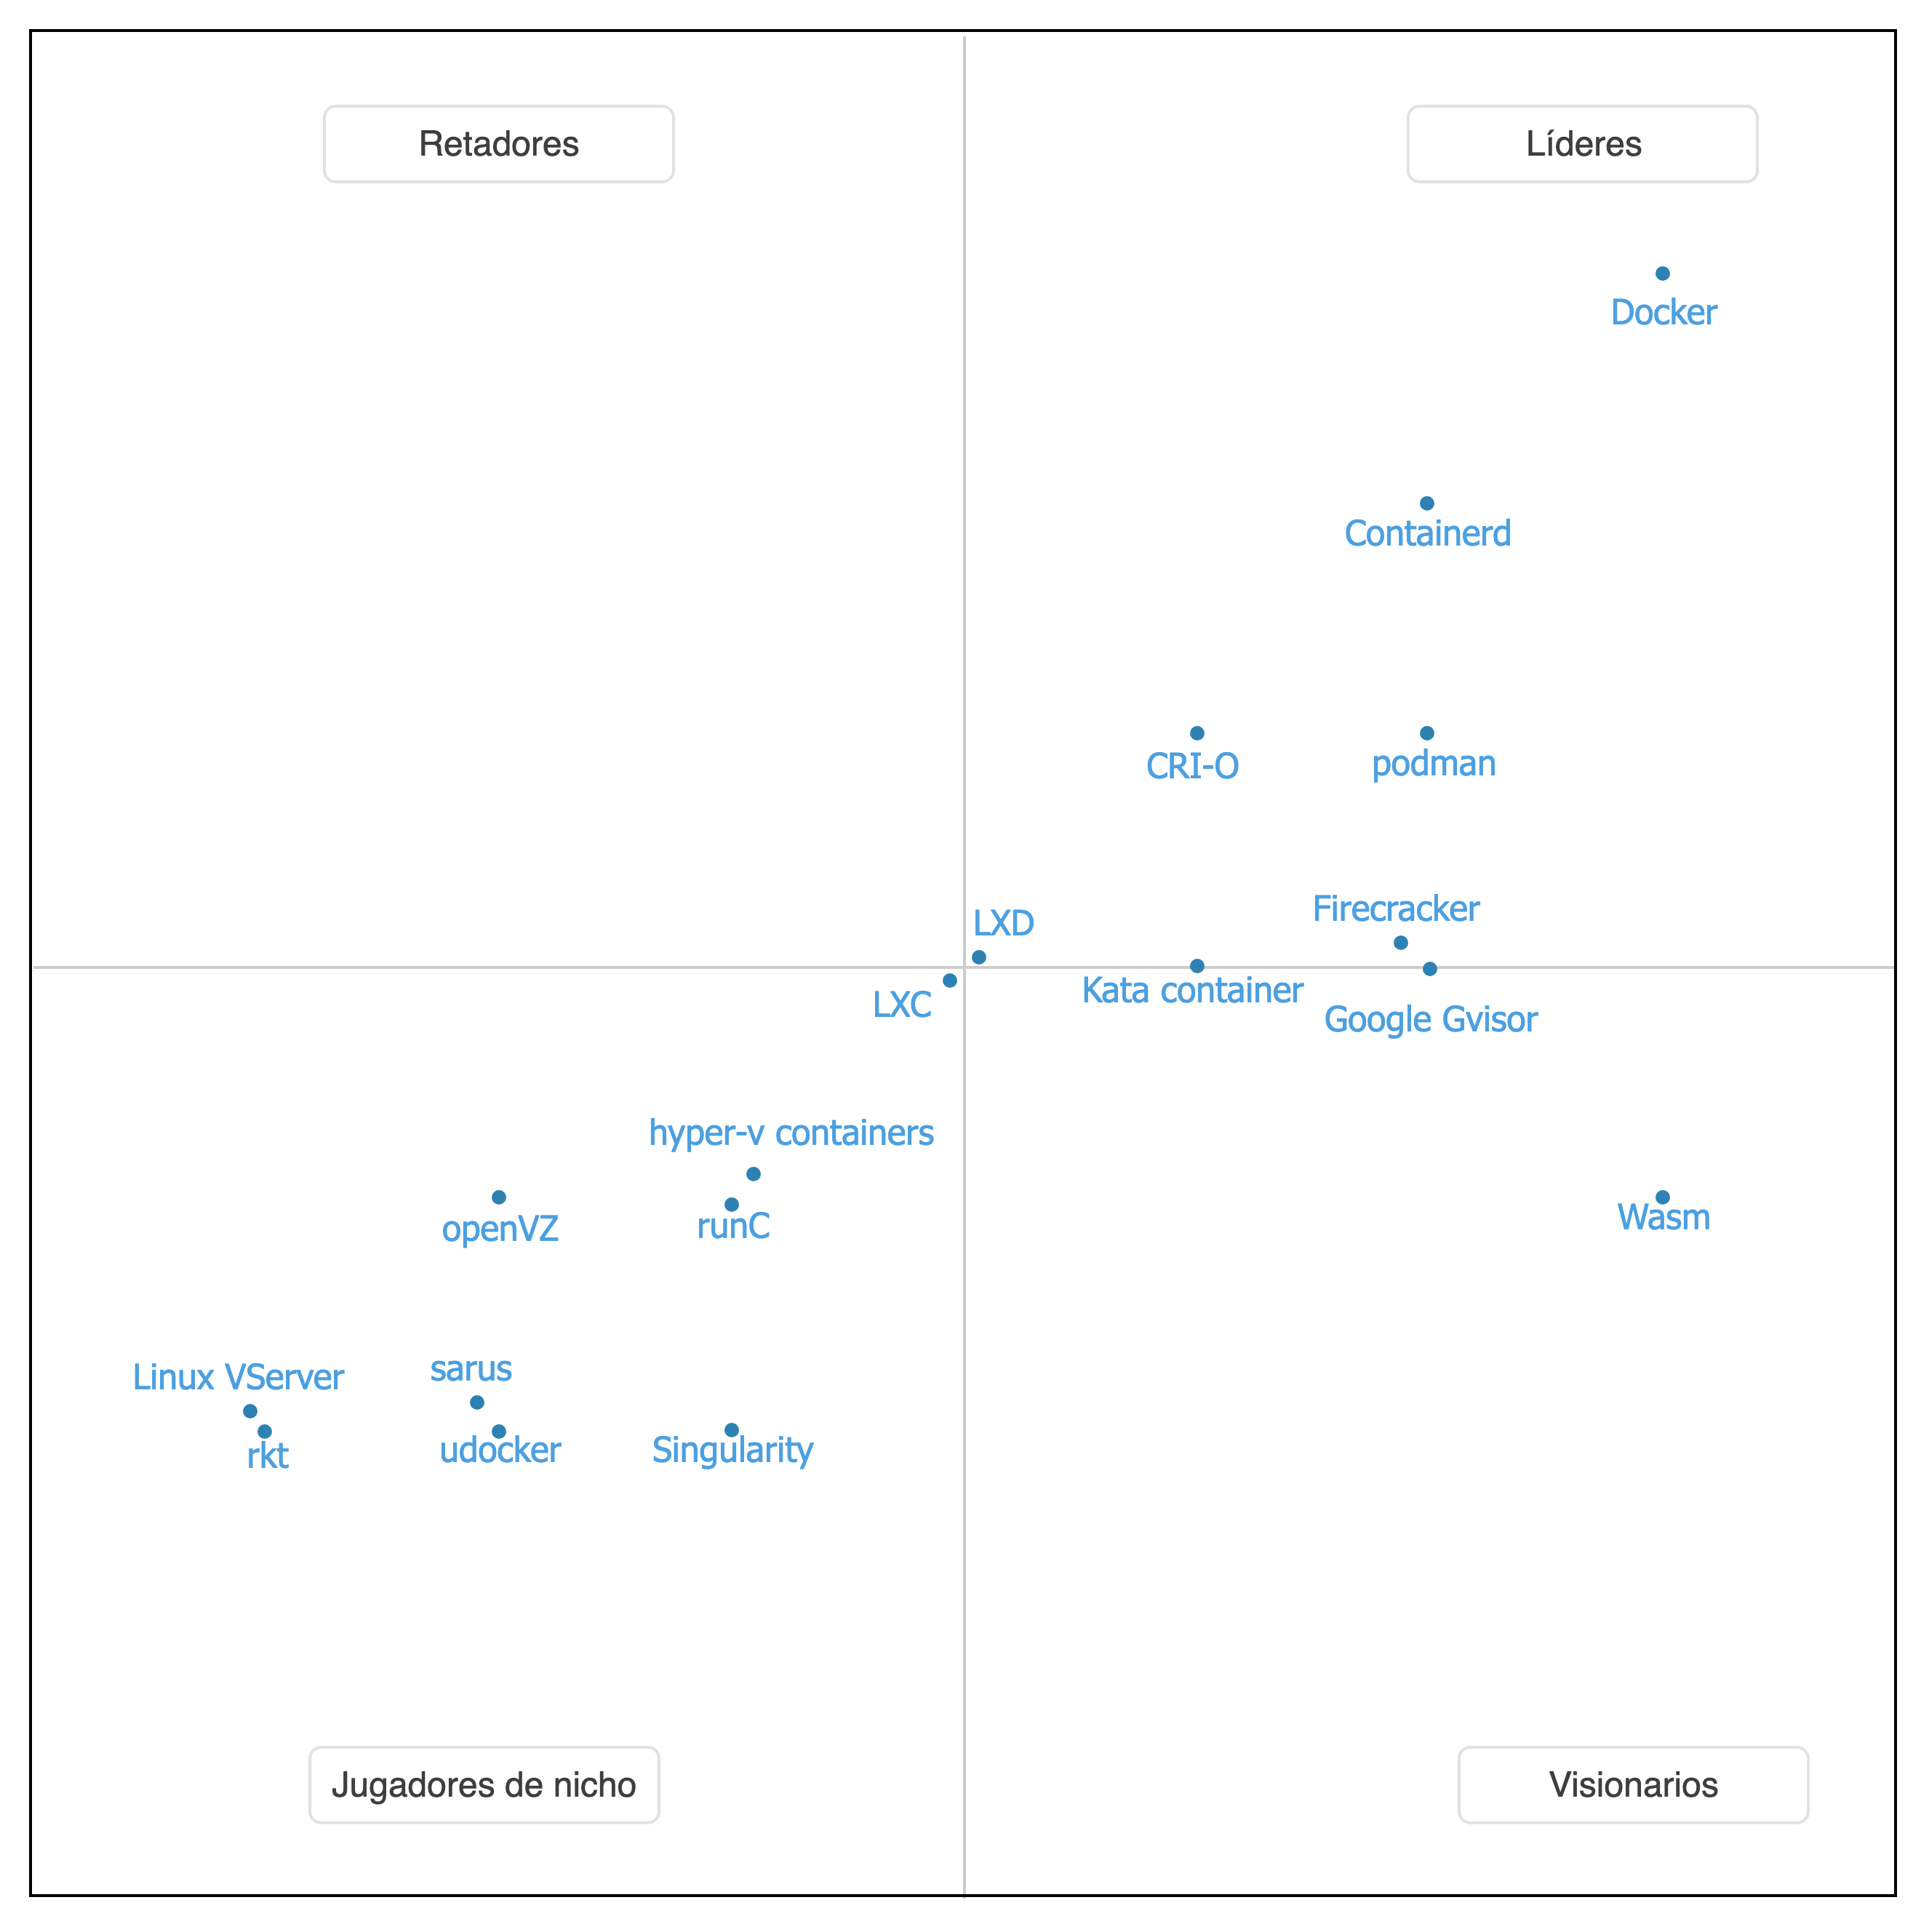
\includegraphics[width=\textwidth] {tablas-images/cp3/cuadrante-gartner.png}
    \caption{Cuadrante de Gartner de cada VBC}\label{fig:tabla-cuadrante-gartner}
\end{figure}
\begin{table}[H]
\centering
\scriptsize
\setlength{\tabcolsep}{3pt}
\renewcommand{\arraystretch}{1.1}
\begin{tabularx}{\textwidth}{|p{0.2\textwidth}|X|}
\hline
\textbf{Tecnología} & \textbf{Ambiente de Ejecución} \\
\hline
Docker & Sistemas Linux, Windows y macOS. Entornos de desarrollo, pruebas y producción, incluyendo la nube pública (\AWS, Google Cloud, Azure). \\
\hline
Podman & Sistemas Linux y macOS, con soporte experimental en Windows. Usado en entornos de desarrollo y producción sin necesidad de un daemon. \\
\hline
Udocker & Sistemas Linux, en entornos de computación de alto rendimiento (\HPC) y servidores compartidos, permitiendo ejecutar contenedores sin privilegios de root. \\
\hline
Wasm (WebAssembly) & Navegadores web (Chrome, Firefox, Safari, Edge). Ejecución en aplicaciones web y entornos de alto rendimiento sin dependencia del sistema operativo subyacente. \\
\hline
LXC & Sistemas Linux. Utilizado para crear contenedores ligeros que actúan como máquinas virtuales, con aplicaciones aisladas en servidores y plataformas de nube privada. \\
\hline
Containerd & Sistemas Linux y Windows. Usado en plataformas de orquestación como Kubernetes, y en infraestructuras de contenedores a gran escala. \\
\hline
LXD & Sistemas Linux. Virtualización ligera de contenedores como máquinas virtuales completas, ideal para servidores y plataformas de virtualización en la nube privada. \\
\hline
Rkt & Sistemas Linux. Anteriormente usado en entornos de orquestación de contenedores y en infraestructuras de nube privada. (Descontinuado actualmente). \\
\hline
Singularity & Sistemas Linux, especialmente en entornos de computación científica y \HPC\ . Portabilidad de aplicaciones científicas sin necesidad de privilegios de root. \\
\hline
runC & Sistemas Linux. Runtime ligero de contenedores compatible con los estándares de la Open Container Initiative (\OCI), utilizado por plataformas como Docker y Kubernetes. \\
\hline
CRI-O & Sistemas Linux. Integrado con Kubernetes para la gestión eficiente de contenedores en plataformas de orquestación en la nube y servidores locales. \\
\hline
Hyper-V containers & Sistemas Windows (Windows Server y Windows 10 con Hyper-V habilitado). Usado para contenedores con aislamiento mediante micro-VMs, ideal para entornos híbridos. \\
\hline
OpenVZ & Sistemas Linux. Virtualización a nivel de contenedor en proveedores de hosting para ofrecer entornos aislados y eficientes. \\
\hline
Linux VServer & Sistemas Linux. Contenedores que funcionan como servidores virtuales, usados en entornos de hosting y administración de servidores de alta disponibilidad. \\
\hline
Google gVisor & Plataformas de nube, especialmente Google Cloud. Capa adicional de seguridad para contenedores en entornos multitenant. \\
\hline
Kata Containers & Sistemas Linux. Virtualización ligera con aislamiento similar a máquinas virtuales, utilizado en plataformas de contenedores en la nube y servidores donde se requiere seguridad. \\
\hline
Firecracker & Plataformas de computación en la nube, como \AWS\ . Optimizado para micro-VMs ultra ligeras y de alto rendimiento en entornos serverless. \\
\hline
Sarus & Sistemas Linux. Entornos de computación de alto rendimiento (\HPC) y clústeres de supercomputación, proporcionando portabilidad y eficiencia sin privilegios de root. \\
\hline
\end{tabularx}
\caption{Entornos de ejecución de cada VBC}
\label{tab:entornos-ejecucion-vbc}
\end{table}
\begin{table}[H]
\centering
\scriptsize
\setlength{\tabcolsep}{4pt}
\renewcommand{\arraystretch}{1.2}
\begin{tabularx}{\textwidth}{|X|X|}
\hline
\textbf{Fortalezas} & \textbf{Oportunidades} \\
\hline
\begin{minipage}[t]{\linewidth}
\vspace{2pt}
\begin{itemize}
    \setlength\itemsep{0pt}
    \setlength\parskip{0pt}
    \setlength\parsep{0pt}
    \item La VBC es ampliamente utilizada en plataformas en la nube como AWS, Azure y Google Cloud.
    \item Herramientas como Kubernetes y Docker se actualizan constantemente, agregando nuevas funcionalidades y mejoras.
    \item Numerosos foros, grupos y organizaciones están dedicados a mejorar y desarrollar soluciones de contenerización.
    \item Los contenedores pueden ejecutarse en múltiples entornos (local, nube, híbrido).
    \item Permiten una mejor utilización de recursos en comparación con las máquinas virtuales tradicionales.
\end{itemize}
\vspace{2pt}
\end{minipage}
&
\begin{minipage}[t]{\linewidth}
\vspace{2pt}
\begin{itemize}
    \setlength\itemsep{0pt}
    \setlength\parskip{0pt}
    \setlength\parsep{0pt}
    \item Los contenedores son ligeros y comparten el kernel del sistema operativo, reduciendo el consumo de recursos.
    \item Una aplicación en contenedor puede ejecutarse en cualquier entorno compatible sin modificaciones.
    \item Permiten implementar y gestionar aplicaciones de manera escalable y eficiente.
    \item Los contenedores permiten que las aplicaciones se ejecuten de manera independiente, evitando conflictos entre ellas.
    \item Herramientas como Docker Compose y Kubernetes facilitan la gestión automatizada de contenedores.
\end{itemize}
\vspace{2pt}
\end{minipage}
\\
\hline
\textbf{Debilidades} & \textbf{Amenazas} \\
\hline
\begin{minipage}[t]{\linewidth}
\vspace{2pt}
\begin{itemize}
    \setlength\itemsep{0pt}
    \setlength\parskip{0pt}
    \setlength\parsep{0pt}
    \item Los contenedores comparten el mismo núcleo del sistema operativo host, lo que podría permitir que una vulnerabilidad afecte a todos los contenedores.
    \item A medida que crece la infraestructura, gestionar múltiples contenedores y sus redes se vuelve complejo.
    \item A diferencia de las máquinas virtuales tradicionales, los contenedores son efímeros por diseño, lo que complica el manejo de datos persistentes.
    \item No todos los sistemas y aplicaciones son compatibles de manera nativa con contenedores, lo que requiere configuraciones específicas.
    \item La seguridad y rendimiento de los contenedores están directamente relacionados con el sistema operativo subyacente.
\end{itemize}
\vspace{2pt}
\end{minipage}
&
\begin{minipage}[t]{\linewidth}
\vspace{2pt}
\begin{itemize}
    \setlength\itemsep{0pt}
    \setlength\parskip{0pt}
    \setlength\parsep{0pt}
    \item Si no se aplican buenas prácticas, los contenedores pueden ser vulnerables a ataques.
    \item El uso de soluciones propietarias como AWS o Azure puede generar dependencia tecnológica.
    \item Las tecnologías de contenerización evolucionan rápidamente, lo que puede dejar obsoletas algunas soluciones.
    \item Un mal diseño puede llevar a un consumo ineficiente de recursos.
    \item Aunque existen buenas prácticas, no hay una regulación estándar única para la gestión de contenedores.
\end{itemize}
\vspace{2pt}
\end{minipage}
\\
\hline
\end{tabularx}
\caption{Tabla de matriz DOFA para el cuadrante gartner}
\label{tab:matriz-dofa}
\end{table}
\begin{table}[H]
\centering
\rowcolors{2}{gray!10}{white}
\begin{tabularx}{\textwidth}{>{\raggedright\arraybackslash}X >{\raggedright\arraybackslash}X}
\rowcolor{gray!30}
\textbf{Tecnología} & \textbf{Enlace a la Documentación} \\

Docker & \href{https://docs.docker.com/}{link} \\
Podman & \href{https://podman.io/docs}{link} \\
Udocker & \href{https://github.com/indigo-dc/udocker}{link} \\
Wasm (WebAssembly) & \href{https://webassembly.org/docs/faq/}{link} \\
LXC & \href{https://linuxcontainers.org/incus/docs/main/}{link} \\
Containerd & \href{https://containerd.io/docs/}{link} \\
LXD & \href{https://linuxcontainers.org/incus/docs/main/}{link} \\
Rkt & \href{https://github.com/rkt/rkt}{link} \\
Singularity & \href{https://docs.sylabs.io/guides/4.3/user-guide/}{link} \\
runC & \href{https://github.com/opencontainers/runc}{link} \\
CRI-O & \href{https://github.com/cri-o/cri-o}{link} \\
Hyper-V containers & \href{https://docs.microsoft.com/en-us/virtualization/windowscontainers/}{link} \\
OpenVZ & \href{https://openvz.org/}{link} \\
Linux VServer & \href{http://linux-vserver.org/Documentation}{link} \\
Google gVisor & \href{https://gvisor.dev/docs/}{link} \\
Kata Containers & \href{https://katacontainers.io/docs/}{link} \\
Firecracker & \href{https://firecracker-microvm.github.io/}{link} \\
Sarus & \href{https://github.com/eth-cscs/sarus}{link} \\

\end{tabularx}
\caption{Enlaces a la documentación de tecnologías de contenerización}
\end{table}